\documentclass[12pt]{article}
\usepackage{lingmacros}
\usepackage{tree-dvips}
\usepackage[utf8]{inputenc}
\usepackage[russian]{babel}
\usepackage{amsmath,amssymb}
\usepackage{multirow}
\usepackage{hyperref}
\usepackage{caption}
\usepackage{tabularx}

\usepackage{graphicx}
\graphicspath{ {./images/} }

\usepackage{listings}
\usepackage{color}

\definecolor{dkgreen}{rgb}{0,0.6,0}
\definecolor{gray}{rgb}{0.5,0.5,0.5}
\definecolor{mauve}{rgb}{0.58,0,0.82}
\definecolor{orange}{rgb}{1,0.6,0}

\lstset{frame=tb,
  language=C++,
  aboveskip=1mm,
  belowskip=1mm,
  showstringspaces=false,
  columns=flexible,
  basicstyle={\small\ttfamily},
  numbers=none,
  numberstyle=\color{orange},
  keywordstyle=\color{blue},
  commentstyle=\color{dkgreen},
  stringstyle=\color{mauve},
  breaklines=true,
  breakatwhitespace=true,
  tabsize=3
}

\begin{document}
\title{Lowest Common Ancestor. Sprase Table}
\date{}
\maketitle

\section*{Дефиниция и примери}
\subsection*{Дефиниция}
\paragraph*{}
Нека имаме кореново дърво $T$ с корен $root$. Връх $u$ се нарича предшественик на връх $v$, ако $u$ лежи на единствения път между $root$ и $v$. Ще бележим с $depth(u)$ дълбочината на връх $u$ или с други думи казано - разстоянието от $root$ до $u$. При тази конвенция, най-близкият общ предшественик на $u$ и $v$, който ще бележим с $lca(u, v)$, ще бъде върхът $x$ с максимална дълбочина, който е предшественик едновременно на $u$ и $v$. 
\subsection*{Примери}
\paragraph*{}
В този случай коренът е връх 1.

\begin{figure}[h]
\caption*{Фигура 1}
\centering
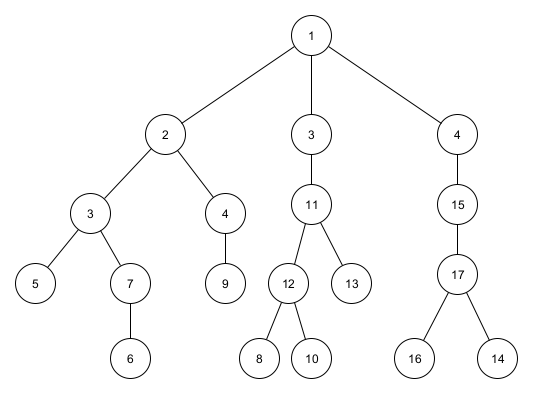
\includegraphics[width=0.5\textwidth]{tree1}
\end{figure}

\raggedright
\begin{itemize}
	\item $lca(5, 7) = 3$;
	\item $lca(4, 9) = 4$;
	\item $lca(3, 9) = 2$;
	\item $lca(2, 13) = 1$;
	\item $lca(4, 14) = 4$;
	\item $lca(2, 4) = 1$;
\end{itemize}

\section*{Свойства на lca(u, v)}
\begin{itemize}
	\item $lca(u, v) = lca(v, u)$
	\item $lca(u, v) = u$ тогава и само тогава, когато u e предшественик на $v$
	\item $lca(u, lca(v, w)) = lca(lca(u, v), w)$.
\paragraph*{}
По тази причина можем да записваме обобщено $lca(u, v, w)$. Това е полезно, ако например имаме нужда да пресмятаме $lca$ на цели интервали от масив. Поради това свойство знаем, че задачата има смисъл и може да се реши със сегментно дърво. От следващото свойство ще научим, че има и по-добър начин.
	\item $lca(u, v, v) = lca(u, v)$
\paragraph*{}
Това значи, че добавянето на "излишни" върхове към тези, на които търсим $lca$ не променя отговора. Тост ако искаме да сметнем $lca$ на група върхове можем да си ползволим да сметнем $lca$ на група, която съдържа тези върхове, но по няколко пъти. Това ни дава възможност да пресмятаме $lca$ на интервал от върхове чрез sparse table. Повече по темата ще научите по-късно.
	\item $lca(u, v) = lca(u, v')$, където $v'$ се получава, когато "качим" връх $v$ на нивото на връх $u$ (разбира се, приемаме, че $depth(u) \leq depth(v)$)
	\item $depth(lca(u, v)) \leq depth(u)$ и $depth(lca(u, v)) \leq depth(v)$.
\paragraph*{}
Можете да се убедите с примери от Фигура 1:
\begin{itemize}
	\item u = 5, v = 6, v' = 7
	\item u = 2, v = 13, v' = 3
	\item u = 11, v = 14, v' = 15
	\item u = 2, v = 9, v' = 2
\end{itemize} 
Тук ще покажем не съвсем формално доказателство на свойството. Ясно е, че след като само "покачваме" връхове то няма как $lca$ да "слезе". Затова само трябва да проверим, че $lca(u, v)$ е предшественик на $u$ и $v'$. Нека запишем $l = lca(u, v)$, тривиално е, че $l$ предшества $u$. Сега трябва да видим дали предшества $v'$. Допускаме противното: нека $l$ не предшества $v'$. Ние знаем, че $l$ предшества $v$. Тъй като ние само сме се качвали нагоре, то единственият вариант $l$ вече да не предшества $v'$ е да сме го "подминали", тоест $l$ да лежи на пътя между $v$ и $v'$. Ясно е също и че $l \neq v'$. Това обаче е противоречие, понеже $depth(l) \leq depth(u) = depth(v') \leq depth(v)$ и излиза, че няма как $l$ да лежи на пътя между $v$ и $v'$.
\end{itemize}

\section*{LCA с binary lifting}
\paragraph*{}
Използвайки тези свойства можем да изготвим алгоритъм, който намира $lca(u, v)$ за $O(logN)$. 
\paragraph*{}
Забелязваме, че ако имаме два върха $u$ и $v$ на равна дълбочина, то ако започнем постепенно да ги "качваме" едновременно, то стойностите ще се различават до един момомент и по-конкретно, първата стойност на съвпадение ще бъде точно $lca(u, v)$. Нека имаме функция $rise(u, n)$, която връща връх, отговарящ на връх $u$ след като бъде "качен" с $n$ стъпки. Тоест така излиза, че трябва да намерим най-малкото $n$, за което $rise(u, n) = rise(v, n)$ и тази стойност ще бъде $lca(u, v)$. По-късно обаче, ще стане ясно, че е по-добре да намерим последното $n$, за което $rise(u, n) \neq rise(v, n)$ и така $lca(u, n)$ ще бъде $parent(rise(u, n))$, където $paret(x)$ е родителят на $x$.
\paragraph*{}
От тези наблюдения става ясно, че е доста удобно да имаме бърз начин да "качваме" връхове. По тази причина е измислена техниката binary lifting. Идеята е следната: за всеки връх $x$ пазим $rise(x, 1)$, $rise(x, 2)$, $rise(x, 4)$, ..., $rise(x, 2^k)$, ... (разбира се няма нужда да пазим тези стойности до безкрай, а само до достатъчно голяма степен на 2). Ключовото наблюдение тук е, че тези стойности могат да се пресмятат доста лесно. Например: $rise(x, 1) = parent(x)$. Също така $rise(x, 2) = parent(parent(x)) = rise(rise(x, 1), 1)$. Забелязваме също и че: $rise(x, 2^k) = rise(rise(x, 2^{k-1}), 2^{k-1})$. Това е вярно, понеже искаме да направим $2^k$ стъпки нагоре, които можем да разделим на два скока по $2^{k-1}$. Разбира се, че ако се опитаме да скочим прекалено нагоре, няма да има връх в дървото, който да отговаря на този скок. Например $rise(2, 2)$ в дървото от Фигура 1 не съществува. Затова за такива случаи записваме, че стойността е $-1$. Също така приемаме, че $rise(-1, 2^k) = -1$.  Сега можем да разширим способностите на нашата функция $rise$. Забелязваме, че ако можем да представим число като сума от степени на двойката, то можем и да направим подходяща поредица от изкачвания, с които да постигнем скок с исканата големина. Например, ако искаме да пресметнем $rise(x, 7)$ можем да използваме $rise(rise(rise(x, 1), 2), 4)$. Тоест, като използваме, че $7=4+2+1$, то правим първо скок с дължина 1, после скок с дължина 2 и накрая скок с дължина 4. Друг пример е: $rise(x, 10) = rise(rise(x, 2), 8)$.
\paragraph*{}
Имайки тези знания можем да направим алгоритъм, който може да намира $lca$ на два върха $u$ и $v$. Допускаме, че $dept(u) \leq depth(v)$. Първо можем да изравним дълбочината на двата върха за $O(logN)$ и така ще трябва да смятаме $lca$ на два върха с еднаква дълбочина. Нека новата стойност на $v$ след изравняването бъде $v'$. Тогава знаем, че същестува $n$, за което $rise(u, n) \neq rise(v', n)$ и $rise(u, n+1) = rise(v', n+1)$. Тоест искаме да намерим последното $n$, за което някакво си условие е в сила. В такива ситуации можем да направим нещо като binary search по битовете на $n$ и да се опитваме да правим старши битове да бъдат $1$ без да разваляме свойството. По-конкретно, тръгваме да ходим по битовете на числото в обратен ред $MAXBit, MAXBit-1, MAXBit-2, ..., 2, 1, 0$ и за всеки бит $b$ проверяваме дали $rise(u, n+2^b) \neq rise(v', n+2^b)$, ако да, то $n += 2^b$ ($n$ започва от $0$). За повече детайли вижте имплементацията.  	

\subsection*{Имплементация}
\paragraph*{}
Имплементацията на lca with bynary lifting е също доста проста, както и идеята. Грубо казано, след като имаме определен корен на дървото ще пуснем едно $dfs$, което да инициализира родителите и дълбочините на върховете. Също трябва да попълним стойностите за скоковете нагоре в дървото, което може да се направи лесно, ако ги пазим в таблица. Тук е изложена и примерна имплементация.  

\begin{lstlisting}
#include <iostream>
#include <vector>

using namespace std;

const int MAXN = 1e5;
const int MAXLog = 20;

int n;
vector <int> graph[MAXN];

int parent[MAXN], depth[MAXN];
int sparse[MAXLog+2][MAXN];

void dfs(int x, int last, int level)
{
    parent[x] = last;
    depth[x] = level;

    for(int y: graph[x])
    {
        if(y!=last)
            dfs(y, x, level+1);
    }
}

void init(int root)
{
    dfs(root, -1, 1);
    for(int x = 1;x<=n;x++) sparse[0][x] = parent[x];

    for(int l = 1;l<=MAXLog;l++)
    {
        for(int x = 1;x<=n;x++)
        {
            if(sparse[l-1][x]==-1)
                sparse[l][x] = -1;
            else
                sparse[l][x] = sparse[l-1][sparse[l-1][x]];
        }
    }
}

int rise(int x, int levelDiff)
{
    for(int bit = 0;bit<=MAXLog;bit++)
    {
        if(((levelDiff>>bit)&1)==1)
        {
            if(x!=-1)
                x = sparse[bit][x];
        }
    }

    return x;
}

int lca(int u, int v)
{
    if(depth[u]>depth[v])
        swap(u, v);

    v = rise(v, depth[v]-depth[u]);
    if(u==v) return u;

    for(int l = MAXLog;l>=0;l--)
    {
        if(sparse[l][u]!=sparse[l][v])
        {
            u = sparse[l][u];
            v = sparse[l][v];
        }
    }

    return parent[u];
}

int main()
{
    cin >> n;
    for(int i = 0;i<n-1;i++)
    {
        int a, b;
        cin >> a >> b;

        graph[a].push_back(b);
        graph[b].push_back(a);
    }

    int root;
    cin >> root;

    init(root);
}

\end{lstlisting}

\section*{Приложение на LCA}
\subsection*{Пътища в дърво}
\paragraph*{}
Единственият път от $u$ до $v$ в дърво е точно пътят $u \rightarrow lca(u, v) \rightarrow v$. Тоест от $u$ се качваме до $lca(u, v)$ и след това от там слизаме до $v$. 
\subsection*{Проверка за положение на върхове}
\paragraph*{}
Можем да проверим дали връх $u$ e предшественик на връх $v$, ако проверим дали $lca(u, v)$ е равно на $u$.

\section*{Задачи за LCA}
\subsection*{Открито първенство на София по информатика 2020 - В2 Пътища}
\paragraph*{}
\href{https://arena.olimpiici.com/#/catalog/533/problem/1326}{Условие на задачата}
\paragraph*{}
\href{https://www.youtube.com/watch?v=C1oz4oq7YWc}{Анализ}

\subsection*{Codeforces - Hill Climbing}
\paragraph*{}
\href{https://codeforces.com/problemset/problem/406/D}{Условие и анализ на задачата}

\section*{LCA с Euler Tour}
\paragraph*{}
\href{https://cp-algorithms.com/graph/lca.html}{Tutorial от cp-algorithms}
\subsection*{Euler Tour}
\paragraph*{}
Euler tour или Ойлерово обхождане е начин за обхождане на дърво базиран на DFS. Идеята е, че коренът на поддърво стои в началото и края на подмасива, който представлява поддървото, а също така и между всеки два подмасива, отговарящи за някое поддърво на поддървото. По-конкретно, примерна имплементация на алгоритъма е следната.

\begin{lstlisting}
void dfs(int x, int last, vector <int> &eulerTour)
{
    eulerTour.push_back(x);
    for(int y: adj[x])
    {
        if(y!=last)
        {
            dfs(y, x, eulerTour);
            eulerTour.push_back(x);
        }
    }
}
\end{lstlisting}

\begin{figure}[h]
\caption*{Фигура 2}
\centering
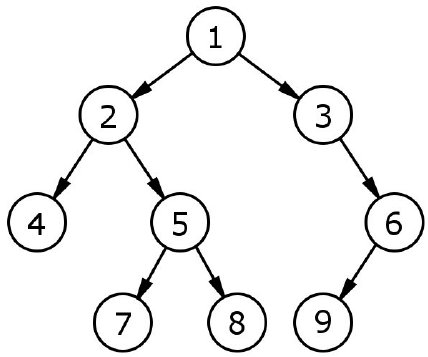
\includegraphics[width=0.5\textwidth]{tree2}
\end{figure}

\paragraph*{}
Ето как би изглеждало едно примерно Ойлерово обхождане на дървото от Фигура 2. Тук сме показали и дълбочината на върха, понеже тя ще е важна по-късно.
\paragraph*{}
\begin{tabular}{ |c|c|c|c|c|c|c|c|c|c|c|c|c|c|c|c|c|c| } 
\hline
ind & 0 & 1 & 2 & 3 & 4 & 5 & 6 & 7 & 8 & 9 & 10 & 11 & 12 & 13 & 14 & 15 & 16 \\
\hline
vertex & 1 & 2 & 4 & 2 & 5 & 7 & 5 & 8 & 5 & 2 & 1 & 3 & 6 & 9 & 6 & 3 & 1 \\ 
\hline
depth & 0 & 1 & 2 & 1 & 2 & 3 & 2 & 3 & 2 & 1 & 0 & 1 & 2 & 3 & 2 & 1 & 0 \\
\hline
\end{tabular}

\paragraph*{}
Оказва се, че ако искаме да намерим lca на два върха $u$ и $v$ трябва да намерим върха, който е с най-малка дълбочина и се намира между първите срещания на тези върхове. Първото срещане на връх $u$  e индексът, на който връх $u$ се среща за пръв път в ойлеровото обхождане. Можете да се убедите с примери. Грубо идеята е, че $lca$ е най-високият връх на пътя между два връха, а този интервал, който се получава че разглеждаме съдържа път, който може да не е прост, но е не се "изкачва" прекалено много. Откриването на този връх може да стане по много начини - с коренова декомпозиция, сегментно дърво и т.н., но ние ще се спрем на имплементацията със sprase table, понеже най-често тази комбинация се оказва полезна.

\section*{Sparse table}
\paragraph*{}
\href{https://cp-algorithms.com/data_structures/sparse-table.html}{Tutorial от cp-algorithms}
\paragraph*{}
Подобно на кореновата декомпозиция и сегментните дървета, sprase table-а също пази определена информация от търсения вид за разни интервали от нашия масив. По-конкретно, нека приемем, че ще търсим минимум в интервал. Нека имаме масив $a[]$ с размер $n$. Тогава sparse table-a $sparse[j][i]$ ще пази минимума за интервала $[i, i+2^j-1]$. Разбира се няма нужда да използваме стойности за $j$ по-големи от $log_2(n)$. Също така, ако се окаже, че $i+2^j-1 \geq n$ (тоест излиза от масива), тогава $sparse[j][i]$ ще пази минимум само за елементите до края на масива (един вид си представяме, че след края има безброй неутрални елементи спрямо операцията, която извършваме, в случая на $min$ този елемент е $+\infty$). Забелязваме също, че можем лесно да пресмятаме стойностите на $sparse[i][j]$. В общия случай, когато не излизаме от масива $sparse[j][i] = min(sparse[j-1][i], sparse[j-1][i+2^{j-1}])$. Така можем да пресметнем всички нужни ни стойности. Ето една примерна имплементация. 
\begin{lstlisting}
for(int i = 0;i<n;i++) sparse[0][i] = a[i];
for(int l = 1;l<=MAXLog;l++)
{
	for(int i = 0;i<n;i++)
	{
		if(i+(1<<(l-1)) >= n)
			sparse[l][i] = sparse[l-1][i];
		else
			sparse[l][i] = min(sparse[l-1][i], 
			                     sparse[l-1][i+(1<<(l-1))]);
	}
}
\end{lstlisting}

\paragraph*{}
Другият въпрос, който остава е как да правим query в тази структура. Обръщаме внимание, че sparse table работи само при оператори, които са идемпотентни, тоест добавянето на елемент по няколко пъти към "сметката" не я променя. По-конкретно, всички знаем, че $min(a, b) = min(a, b, a)$. Тоест като добавим елемент няколко пъти, стойността се запазва. Това важи за функции като $lca$, $gcd$(НОД), $lcm$(НОК), $max$ и други. Обръщаме внимание, че не важи за сума, тоест $sum(a, b) \neq sum(a, b, a)$ в общия случай.
\paragraph*{}
Връщайки се към конкретната задача: как да намираме $min$ за числата в интервала $[l, r]$ бързо. Забелязваме, че интервала може да се покрие от два интервала, които имат размер точна степен на двойката, по-конкретно $sz = 2^{[log_2(r-l+1)]}$, нека отбележим цялата част на двоичния логаритъм със $L = [log_2(r-l+1)]$. Така минимумът за един интервал е точно $min(sparse[L][l], sparse[L][r-2^L+1])$. Обърнете внимание, че тези два интервала могат да се пресичат. Това е и причината да изискваме идемпотентност.   
\paragraph*{}
Цялата на част на двоичния логаритъм можем предварително да precompute-нем по такъв начин.

\begin{lstlisting}
log2[1] = 0;
for(int x = 2;x<=MAXN;x++)
    log2[x] = log2[x/2] + 1;
\end{lstlisting}

\paragraph*{}
Ето и една примерна реализация за RMQ (range minimum query).
\begin{lstlisting}
int rmq(int l, int r) //range minimum query
{
    return min(sparse[log2[r-l+1]][l], 
                sparse[log2[r-l+1]][r - (1<<log2[r-l+1]) + 1]);
}
\end{lstlisting}

\subsection*{Цялостен алгоритъм}
\paragraph*{}
След като вече знаем алгоритъмът с Ойлерово обхождане и можем да боравим със sparse table остава само да направим имплементация. С тези инструменти ние можем да решаваме задачата за lca за $O(N logN)$ precompute и $O(Q)$ за отговаряне на всичките $Q$ заявки.
\paragraph*{}
Тъй като тук ние трябва да връщаме чрез sprase table-а не самата минмална стойност на дълбочина, а  върхът, който я "притежава", то можем да постъпим по няколко начина. Единият е да пазим в структура двете информации - връх и дълбочина, и да напишем функция $min$ за тази структура (може и със std::pair без да се занимаваме със специални min функции. Друг вариант е да напишем специална функция, която при вход от два връха $u$ и $v$ да връха този, който има по-малка дълбочина. Това ще бъде и стратегията за тази имплементация. Малка имплементационна подробност е, че размера на ойлеровото обхождане може да бъде двоен на размера на дървото, затова трябва масивите да бъдат по-големи.
\paragraph*{}
Можете да тествате имплементацията си тук: \href{https://judge.yosupo.jp/problem/lca}{Library Checker - Lowest Common Ancestor}
\begin{lstlisting}
#include <iostream>
#include <vector>

using namespace std;

const int MAXN = 5e5;
const int MAXLog = 20;

int n;
vector <int> adj[MAXN+5];

int depth[MAXN+5], firstSeen[MAXN+5];
int sparse[MAXLog+2][MAXN*2+5], log2[MAXN*2+5];

void dfs(int x, int last, int level, vector <int> &eulerTour)
{
    depth[x] = level;
    firstSeen[x] = eulerTour.size();

    eulerTour.push_back(x);
    for(int y: adj[x])
    {
        if(y!=last)
        {
            dfs(y, x, level+1, eulerTour);
            eulerTour.push_back(x);
        }
    }
}

int getShallowerVertex(int u, int v)
{
    if(depth[u]<depth[v]) return u;
    return v;
}

void init(int root)
{
    vector <int> eulerTour;
    dfs(root, -1, 0, eulerTour);

    log2[1] = 0;
    for(int x = 2;x<=2*MAXN;x++)
        log2[x] = log2[x/2] + 1;

    for(int i = 0;i<eulerTour.size();i++) sparse[0][i] = eulerTour[i];
    for(int l = 1;l<=MAXLog;l++)
    {
        for(int i = 0;i<eulerTour.size();i++)
        {
            if(i+(1<<(l-1)) >= eulerTour.size())
                sparse[l][i] = sparse[l-1][i];
            else
                sparse[l][i] = getShallowerVertex(sparse[l-1][i], sparse[l-1][i+(1<<(l-1))]);
        }
    }
}

int rmq(int l, int r) //range minimum query
{
    return getShallowerVertex(sparse[log2[r-l+1]][l], sparse[log2[r-l+1]][r - (1<<log2[r-l+1]) + 1]);
}

int lca(int u, int v)
{
    if(firstSeen[u]>firstSeen[v]) swap(u, v);
    return rmq(firstSeen[u], firstSeen[v]);
}

int main()
{
    ios::sync_with_stdio(false);
    cin.tie(nullptr);

    int Q;
    cin >> n >> Q;
    for(int i = 1;i<n;i++)
    {
        int p;
        cin >> p;

        adj[p].push_back(i);
    }

    init(0);
    while(Q--)
    {
        int u, v;
        cin >> u >> v;

        cout << lca(u, v) << '\n';
    }
}
\end{lstlisting}

\end{document}